%%%%%%%%%%%%%%%%%%%%%%%%%%%%%%%%%%%%%%%%%%%%%%%%%%%%%%%%%%%%%%%%%%%%%%%%%%%%%%%%
%%
%% Uppsala Beamer theme example by Frédéric Haziza <daz@it.uu.se>
%%
%% Describing beamerthemeUppsala version 2008/05/15
%%
%% If you have more than three sections or more than three subsections in at least
%% one section, you might want to use the [hideallsubsections] or
%% [hideothersubsections] switch.  In this case, only the current (sub-) section is
%% displayed in the sidebar and not the full overview.
%%
%% Options are:
%% ===========
%% * hideallsubsections, hideothersubsections
%% * nonumbers,totalnumber
%% * withnav, mylogo
%% * grey
%% * noprogressbar
%%
%% For the sidebar layout:
%% * subsectionsattop, sectionpathattop
%% 
%% Removed
%% =======
%% * sidebarshades
%%
%% Tip
%% ===
%% latex this file to see the theme in action
%%
%%%%%%%%%%%%%%%%%%%%%%%%%%%%%%%%%%%%%%%%%%%%%%%%%%%%%%%%%%%%%%%%%%%%%%%%%%%%%%%%

\documentclass{beamer}
%\documentclass[handout]{beamer}
%\documentclass[notes]{beamer}
%\documentclass[trans]{beamer}

\usetheme[hideothersubsections]{Uppsala}

\usepackage{hyperref}
\usepackage{pgf}
\usepackage{tikz}
\usepgflibrary{arrows}
\usepgflibrary{shapes}
\usetikzlibrary{%
  arrows,%
  calc,%
  fit,%
  patterns,%
  plotmarks,%
  shapes.geometric,%
  shapes.misc,%
  shapes.symbols,%
  shapes.arrows,%
  shapes.callouts,%
  shapes.multipart,%
  shapes.gates.logic.US,%
  shapes.gates.logic.IEC,%
  er,%
  automata,%
  backgrounds,%
  chains,%
  topaths,%
  trees,%
  petri,%
  mindmap,%
  matrix,%
  calendar,%
  folding,%
  fadings,%
  through,%
  positioning,%
  scopes,%
  decorations.fractals,%
  decorations.shapes,%
  decorations.text,%
  decorations.pathmorphing,%
  decorations.pathreplacing,%
  decorations.footprints,%
  decorations.markings,%
  shadows}

%\usepackage[english]{babel} % or whatever
\usepackage[utf8]{inputenc} % or whatever

\usepackage{mathptmx}
\usepackage{helvet}
%\usepackage{courier}

\usepackage[T1]{fontenc}
% Or whatever. Note that the encoding and the font should match. If T1
% does not look nice, try deleting the line with the fontenc.

\usepackage{cwpuzzle}
\usepackage{astra}

\newcommand{\Dom}[1]{\text{dom}({#1})}
\newcommand{\Table}{\Constraint{Table}}

% SparseBitSet
\newcommand{\Words}{\texttt{words}}
\newcommand{\Index}{\texttt{index}}
\newcommand{\Mask}{\texttt{mask}}
\newcommand{\Limit}{\texttt{limit}}
\newcommand{\SparseBitSet}{\texttt{SparseBitSet}}
\newcommand{\Offset}{\localvar{offset}}

% CT Propagator
\newcommand{\Scp}{\texttt{vars}}
\newcommand{\CurrTable}{\texttt{validTuples}}
\newcommand{\Sval}{\texttt{S^{val}}}
\newcommand{\Ssup}{\texttt{S^{sup}}}
\newcommand{\LastSizes}{\texttt{lastSize}}
\newcommand{\Supports}{\texttt{supports}}
\newcommand{\Residues}{\texttt{residues}}

% Pseduo code
\newcommand{\ForEach}[1]{\textbf{foreach } {#1} \textbf{ do }}
\newcommand{\ForEachTo}[3]{\textbf{foreach } {#1} \textbf{ from } {#2} 
  \textbf{ to } {#3} \textbf{ do }}
\newcommand{\ForEachDownTo}[3]{\textbf{foreach } {#1} \textbf{ from } {#2} 
  \textbf{ downto } {#3} \textbf{ do }}
\newcommand{\Break}{\textbf{break~}}
\newcommand{\While}[1]{\textbf{while~} {#1} \textbf{~do~}}

\renewcommand{\algorithmicfor}{\textbf{Method}}
\renewcommand{\algorithmicdo}{}
\renewcommand{\algorithmicforall}{\textbf{foreach}}
%\renewcommand{\algorithmicwhile}{\textbf{foreach}}

\newcommand{\Func}[2]{\FOR{#1(#2)}}
\newcommand{\FuncRet}[3]{\FOR{#1(#2) \ : \ \textbf{#3}}}
\newcommand{\Endfunc}{\ENDFOR}
\newcommand{\To}{~\bf{to}~}
\newcommand{\Downto}{~{\bf{downto}}~}
\newcommand{\For}[3]{\FOR{${#1} \leftarrow {#2} \To {#3}$ \textbf{do}}}
\newcommand{\ForDown}[3]{\FOR{${#1} \leftarrow {#2} \Downto {#3}$ \textbf{do}}}
\newcommand{\FOREACH}[1]{\FORALL{{#1} \textbf{do}}}
\newcommand{\ENDFOREACH}{\ENDFOR}

\renewcommand{\algorithmiccomment}[1]{\hfill // #1}
\def\PROCEDURE{\item[\textbf{PROCEDURE}]}
\def\FAILED{\textbf{FAILED}}
\def\NOFIX{\textbf{NOFIX}}
\def\FIX{\textbf{FIX}}
\def\SUBSUMED{\textbf{SUBSUMED}}
\def\FAIL{\textbf{FAIL}}
\def\bool{\mathit{bool}}
\def\StatusMessage{\mathit{StatusMessage}}
\def\FindSupport{\textsc{FindSupport}}
\def\RemoveSupport{\textsc{RemoveSupport}}
\def\Extensional{\textsc{Extensional}}
\def\CompactTable{\textsc{CompactTable}}
\def\UpdateTable{\textsc{UpdateTable}}
\def\FilterDomains{\textsc{FilterDomains}}
\def\FixDomains{\textsc{FixDomains}}
\def\InitialiseCT{\textsc{InitialiseCT}}
\def\IndexOfFixed{\mathit{index\_of\_fixed}}


\newcommand{\ITE}[3]{\text{\bf ~if~} #1 \text{\bf ~then~} #2 \text{\bf ~else~} #3 \text{\bf ~endif}}

\newcommand{\function}[1]{\mathrm{#1}}
\newcommand{\localvar}[1]{\mathit{#1}}

\newlength\myindent
\setlength\myindent{2em}
\newcommand\bindent{%
  \begingroup
  \setlength{\itemindent}{\myindent}
  \addtolength{\algorithmicindent}{\myindent}
}
\newcommand\eindent{\endgroup}

\newcommand{\INDSTATE}[1][1]{\STATE\hspace{#1\algorithmicindent}}
\newcommand{\INDRETURN}[1][1]{\STATE\hspace{#1\algorithmicindent}\textbf{return~}}
\newcommand{\INDIF}[2][1]{\STATE\hspace{#1\algorithmicindent}
  \textbf{if~}{#2}\textbf{~then}}
\newcommand{\INDELSE}[1][1]{\STATE\hspace{#1\algorithmicindent}\textbf{else~}}
\newcommand{\INDELSEIF}[2][1]{\STATE\hspace{#1\algorithmicindent}
  \textbf{else if~}{#2}\textbf{~then}}

\newcommand{\CTpaper}[0]{DBLP:conf/cp/DemeulenaereHLP16}

\newcommand{\stressed}[1]{\emph{{\color{red!50}{#1}}}}

%% -----------------------------------------------------------
%% MISC. INFORMATION
%% -----------------------------------------------------------

\title{Implementation and Evaluation of a Compact Table Propagator in Gecode}
%\subtitle{Bachelor's thesis}

\author[Linnea Ingmar | \emph{linnea.ingmar.3244@student.uu.se}] % appears in the footline
{Linnea Ingmar \\ <\texttt{linnea.ingmar.3244@student.uu.se}>}


\institute[Dept. of Information Technology] % appears in the footline
{
  The ASTRA Group\\ on Combinatorial Optimisation \\
  Uppsala University
}


\date[\today] % appears in the bottom of the sidebar
{\today}

%% \logo{...}

%% This is only inserted into the PDF information catalog. Can be left out.
\subject{Unofficial Beamer Theme for Uppsala University}

%% -----------------------------------------------------------
%% Extra ``local'' settings
%% -----------------------------------------------------------

% Comment out this, if you do not want the table of contents to pop up at
% the beginning of each (sub)section:
\AtBeginSection[]
{
  \begin{frame}<beamer> % with <beamer> => doesn't appear in handout mode
    \frametitle{Outline} %% Put the title you want, or none!
    %\tableofcontents[currentsection,currentsubsection]
    \tableofcontents[currentsection]
  \end{frame}
}

%% Unfolds piecewise element with shading.
%% Text appears, shaded, and the audience knows that somehting is coming
%% Note: if you set the number too high, the audience will try to read the 
%% text that now shows up more, and will be disturbed.
%% ``dynamic'' makes elements show gradually more and more.
\setbeamercovered{transparent=5}
%% \setbeamercovered{dynamic=5}

%% -----------------------------------------------------------

\begin{document}

\begin{frame}[plain] %% Gets the frame to fill up the page, no menu/sidebar/footline
  \titlepage
  
  \begin{figure}
    \begin{flushright}
        \begin{tabular}[t,right]{lr}
          Supervisor: & Mats Carlsson (SICS) \\
          Reviewer:   & Pierre Flener
        \end{tabular}
      \end{flushright}
  \end{figure}

\end{frame}

\begin{frame}
    \frametitle{Outline}
    \tableofcontents[currentsection]
\end{frame}

\section{Background}

\subsection{Constraint Programming}
% Kakuro

\begin{frame}
  \frametitle{Kakuro puzzle}
  \begin{minipage}{0.45\textwidth}
    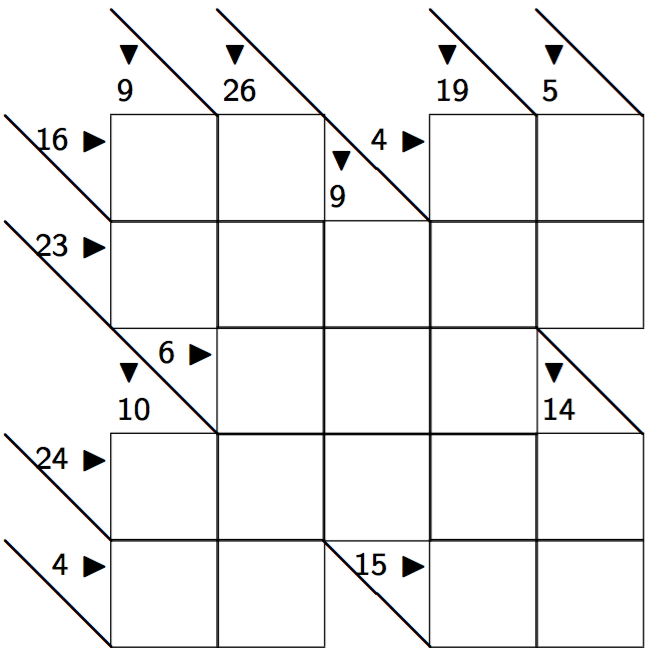
\includegraphics[scale=0.15]{kakuro.png}
  \end{minipage}
  \begin{minipage}{0.45\textwidth}
    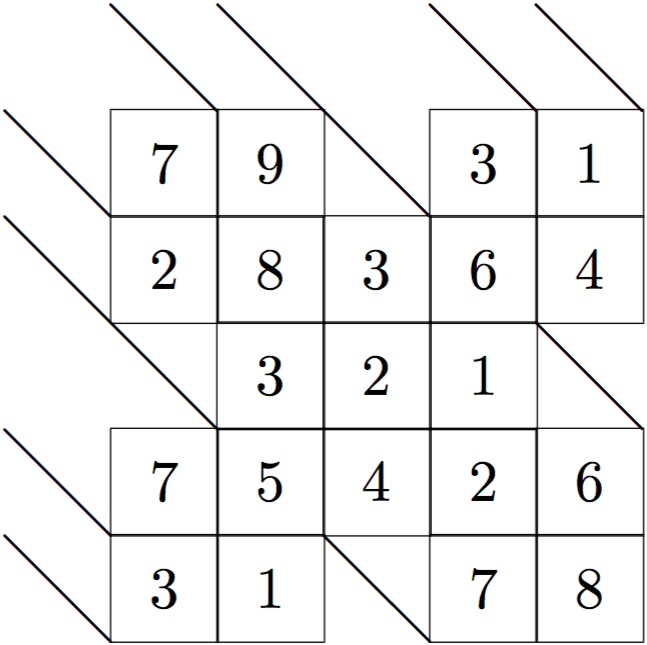
\includegraphics[scale=0.15]{kakuro-sol.png}
  \end{minipage}

  \bigskip

  \begin{itemize}
    \item   Rows and columns of cells (\emph{entries}) with prefilled numbers (\emph{clues}).
    \item   Fill in digits from~$1$ to~$9$ inclusive into the empty cells so that
      for each entry, the sum of the digits is equal to the clue of that entry,
      and so that each digit appears at most once in each entry.
    \end{itemize}

\end{frame}

\begin{frame}
  \frametitle{Kakuro puzzle as a constraint problem (1)}
  \begin{minipage}{0.5\textwidth}
    \begin{description}
      \item[Variables] One per empty cell.
      \item[Domains] $\Set{1...9}$ for all variables.
      \item[Constraints (1)] For each entry: variables are \stressed{distinct},
        and the \stressed{sum} of them is equal to the clue.
    \end{description} 
  \end{minipage}
  \begin{minipage}{0.45\textwidth}
    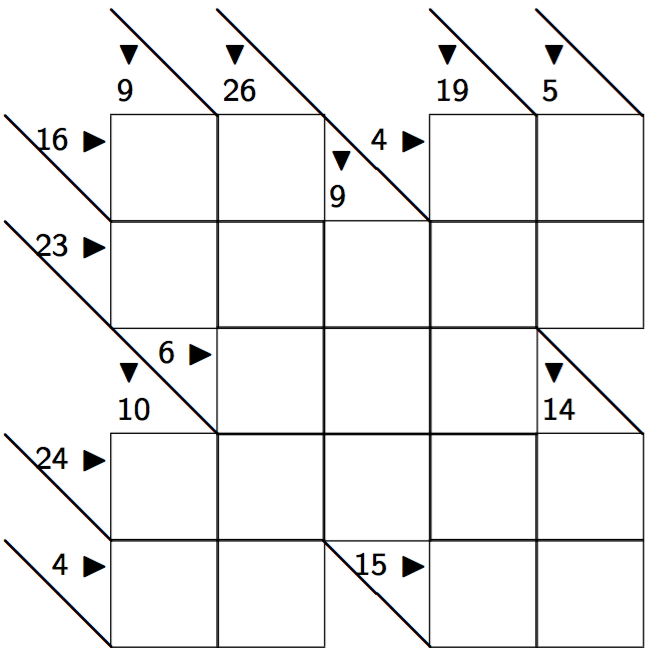
\includegraphics[scale=0.2]{kakuro.png}
  \end{minipage}
\end{frame}

\begin{frame}
  \frametitle{Kakuro puzzle as a constraint problem (2)}
  \begin{minipage}{0.5\textwidth}
    \begin{description}
      \item[Variables] One per empty cell.
      \item[Domains] $\Set{1...9}$ for all variables.
      \item[Constraints (2)] For each entry: state the \stressed{possible
        combinations of values} that the variables can take.
    \end{description} 
  \end{minipage}
  \begin{minipage}{0.45\textwidth}
    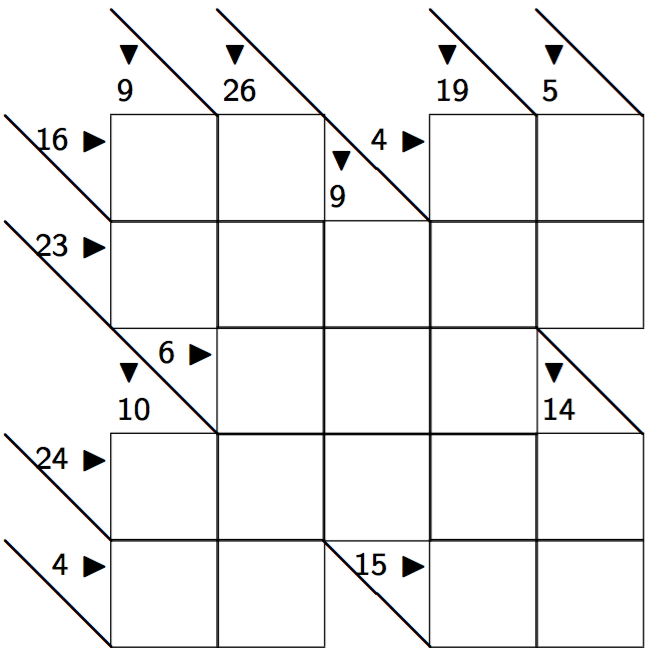
\includegraphics[scale=0.2]{kakuro.png}
  \end{minipage}

  \bigskip
  For an entry of size~$2$ and clue~$4$:~$\Tuple{1,3}$ and~$\Tuple{3,1}$
  are the only combinations.
\end{frame}

% Define:
% - Constraints?
\begin{frame}
  \frametitle{Constraints and \Table~constraints (definitions)}
  \begin{definition}[Constraint]
    \label{def:constraint}
    A \textbf{constraint} on a finite sequene of~$n$ variables~$X$
    is a relation, denoted~$rel(c)$, that
    contains the set of allowed~$n$-tuples for~$X$.
    Each variable~$x_i \in X$ has a corresponding \emph{domain}~$D_i$
    that is the set of possible values that~$x_i$ can take.
  \end{definition}
  
  \begin{definition}[\Table~constraints]
    A \Table~constraint explicitly lists~$rel(c)$ as a sequence
    of~$n$-tuples.
  \end{definition}
  
  Example of a \Table~constraint.

\end{frame}

% - CSP
\begin{frame}
  \frametitle{Constraint Problems (definition)}
  \begin{definition}[Constraint problem]
    A \textbf{constraint satisfaction problem (CSP)} is a 
    triple\\
    \begin{center}
      $\left<V,D,C\right>$\\      
    \end{center}
    where: \\
    \begin{itemize}
      \item $V = v_1, \ldots, v_n$ is a finite sequence of variables,
      \item $D = D_1, \ldots, D_n$ is a finite sequence of domains for the respective variable,
      \item $C = \Set{c_1, \ldots, c_m}$ is a finite set of constraints, 
        each on a subsequence of~$V$.
    \end{itemize}
  \end{definition}
\end{frame}

\begin{frame}
  \frametitle{Constraint Stores (definition)}
  \begin{definition}[Constraint store]
    A \textbf{constraint store}~$s$ is a function mapping a finite set of
    variables~$V = v_1, \ldots, v_n$ to a finite set of domains~$D = D_1, \ldots, D_n$:\\
    \begin{center}
      $s: variables \mapsto domains$
    \end{center}
  \end{definition}
    % We denote the domain of
    % a variable~$v_i$ under~$s$ by~$s(v_i)$ or~$\Dom{v_i}$.
  Furthermore, a store~$s$...

  \begin{itemize}
    \item ...is a \emph{failed store} iff $s(v_i) = \emptyset$ for some~$v_i \in V$.
    \item ...is an \emph{assignment store} iff~$\Cardinality{s(v_i)} = 1$ for all~$v_i \in V$.
    \item ...is a \emph{solution store} for a constraint~$c$ iff~$s$ is an assignment store
      that constructs a solution to~$c$.
  \end{itemize}
\end{frame}

% - Store

\subsection{Propagators}

\begin{frame}
  \frametitle{Propagators (definition)}
  \begin{definition}[Propagators.]
    A \textbf{propagator}~$p$ is a function mapping stores to stores:
    \begin{center}
      $p: store \mapsto store$ 
    \end{center}
  \end{definition}
  Furthermore, a propagator~$p$...
  \begin{itemize}
    \item ...is a decreasing function (i.e. can only remove values and 
      not add new values).
    \item ...is a monotonic function (not a strict obligation).
    \item ...must faithfully implement its constraint.
    \item ...signals a \emph{status message}.
  \end{itemize}
\end{frame}

\begin{frame}
  \frametitle{Status messages}
  \begin{description}
    \item[FAIL.] $p(s)$ is a failed store.
    \item[SUBSUMED.] $p$ can never propagate any more values
      (all the following stores will be fixpoints).
    \item[FIX.] $p(s)$ is a fixpoint to~$p$:~$p(s) = p(p(s))$
    \item[NOFIX.] $p(s)$ is (possibly) not a fixpoint.
  \end{description}

  Obligations regarding status messages:
  \begin{itemize}
    \item Must signal SUBSUMED on a solution store~$s$.
    \item Must signal FAIL on an assignment store~$s$ that is not a solution store.
    \item Must not claim FIX or SUBSUMED if it could propagate more.
  \end{itemize}

  Always safe to signal NOFIX on stores that are not assignment stores.
  
\end{frame}

\subsection{Gecode}

\begin{frame}
  \frametitle{Gecode}
  \textbf{Gecode} (Generic Constraint Development Environment)
  is...

  \begin{itemize}
    \item ...a constraint solver (a software that solves constraint problems).
    \item ...written in C++, modular, extensible, and has state-of-the-art performance.
    \item ...supports the programming of new propagators.
    \item ...developed at KTH, Sweden.
  \end{itemize}

  Two existing propagators for the~\Table~constraint, and one for the 
  related constraint~\Constraint{Regular}, that expresses~$rel(c)$ as a DFA.

\end{frame}

\subsection{The Compact Table algorithm}

\begin{frame}
  % Efficient
  A new propagation algorithm for the~\Table constraint.
  Published in a 2016 paper%~\cite{\CTpaper}.
  No attempt to implement it in Gecode (until now).
\end{frame}

\section{Algorithms}

\subsection{Sparse bit-set}

\subsection{Compact Table}

\begin{frame}
  \begin{algorithm}[H]
    \small
    \begin{algorithmic}[1]
      \PROCEDURE $\CompactTable(s:\text{store}):\Tuple{StatusMsg,\text{store}}$
      \IF{the propagator is being posted}
      \STATE $s \gets \InitialiseCT(s,T_0)$
      \IF{$s = \emptyset$
      }
      \RETURN $\Tuple{\FAIL, \emptyset}$
      \ENDIF
      \ELSE
      \FOREACH{variable~$x \in s$ whose domain has changed since last time}
      \STATE \UpdateTable($s,x$)
      \IF{$\CurrTable$.isEmpty()}
      \RETURN $\Tuple{\FAIL,\emptyset}$
      \ENDIF
      \ENDFOREACH
            \IF{\CurrTable~has changed since last time}
            \STATE $s \gets \FilterDomains(s)$
            \ENDIF
      \ENDIF
      \IF{there is at most one unassigned variable left}
      \RETURN $\Tuple{\SUBSUMED, s}$
      \ELSE 
      \RETURN $\Tuple{\FIX,s}$
      \ENDIF
    \end{algorithmic}
    \caption{Compact Table Propagator.}
    \label{algo:CT}
  \end{algorithm}
\end{frame}

\begin{frame}
  \frametitle{Updating \CurrTable}
  \begin{algorithm}[H]
    \small
    \begin{algorithmic}[1]
        \PROCEDURE \UpdateTable($s$: store, $x$: variable) \label{line:updateTableDelta:1} 
        \STATE $\CurrTable$.clearMask() \label{line:updateTableDelta:4} 
        \IF{$\Delta_x$ is available $\ \land \ |\Delta_x| < |s(x)|$}
          \FOREACH{$a \in \Delta_x$} \label{line:updateTableDelta:5} 
            \STATE $\CurrTable$.addToMask($\Supports[x,a]$) \label{line:updateTableDelta:6} 
          \ENDFOREACH      
          \STATE $\CurrTable$.reverseMask() \label{line:updateTableDelta:7} 
        \ELSE
          \FOREACH{$a \in s(x)$} \label{line:updateTableDelta:8} 
            \STATE $\CurrTable$.addToMask($\Supports[x,a]$) \label{line:updateTableDelta:9} 
          \ENDFOREACH      

        \ENDIF
        \STATE $\CurrTable$.intersectWithMask() \label{line:updateTable:10} 
    \end{algorithmic}
  \end{algorithm}
\end{frame}

\begin{frame}
  \frametitle{Filtering out values}
  \begin{algorithm}[H]
    \small
    \begin{algorithmic}[1]
      \PROCEDURE \FilterDomains($s$) : store
      \FOREACH{$x \in s \text{~such that~} |s(x)| > 1$}
            \FOREACH{$a \in s(x)$}
              \STATE $\localvar{index} \leftarrow \Residues[x,a]$
              \IF{$\CurrTable[index] \ \& \ \Supports[x,a][index] = 0$}
                  \STATE $\localvar{index} \leftarrow \CurrTable$.intersectIndex($\Supports[x,a]$)
                  \IF{$\localvar{index~} \neq -1$}
                        \STATE $\Residues[x,a] \leftarrow \localvar{index}$
                  \ELSE
                        \STATE $s \leftarrow s[x \mapsto s(x) \setminus \Set{a}]$
                  \ENDIF
              \ENDIF
             \ENDFOREACH
      \ENDFOREACH
      \RETURN{$s$}
    \end{algorithmic}
  \end{algorithm}
\end{frame}

\section{Evaluation}
\subsection{Setup}
\subsection{Results}
\subsection{Discussion}

\section{Conclusions}


% \section{Introduction}

% \begin{frame}
%   \frametitle{Why}

%   Why use \LaTeX, when there are specialized presentations tools (OpenOffice.org Impress, Keynote, PowerPoint) available?

%   \begin{itemize}
%     \item{Look: The layout of mathematical formulas and program text is much nicer\ldots not to speak from ligatures in ``ordinary'' text}
%     \item{Reuse of material: Going from a paper to a presentation is easy -- just use the same ``codebase''}
%     \item{Portable solution: You can use whichever operating system you like}
%     \item{Durable solution: usually even very old \LaTeX code can be typeset with modern installations}
%   \end{itemize}

% \end{frame}

% \section{Cool Stuff}

% \begin{frame}
%   \frametitle{Mathematics}

%   \begin{example}
%     \begin{equation}
%       \mathit{Hamming} (X,Y) = \sum_{i=1}^{n} f (x_{i}, y_{i})
%     \end{equation}
%   \end{example}

% with $f(x,y)$ defined as follows:

%   \begin{definition}
%     \begin{equation}
%       f(x,y)= \left\{ \begin{array}{ll}
%           0 & \mbox{iff $|x-y| \leq \epsilon_{h}$,} \\
%           1 & \mbox{else.}      \\
%         \end{array}
%       \right.
%     \end{equation}
%   \end{definition}

% \end{frame}

% \begin{frame}
%   \frametitle{Piecewise Text Modification}

%   \onslide<1>
%     Shown on first slide.
%   \onslide<2>
%     Shown on second slide.
%   \onslide<1>
%     Shown on first slide.
%     \begin{itemize}
%   \onslide<2-3>
%         \item Shown on the second and the third slide.
%   \onslide+<3->
%         \item Shown from slide 3 on.
%     \end{itemize}
%     Shown from slide 3 on.
%   \onslide
%     Shown on all slides.

%     \vskip 1cm
%   \onslide<4>
%     \alert<4>{You get fine-grain control over which elements are visible at each time.}

% \end{frame}

% \begin{frame}
%   \frametitle{Using Ti\textit{k}Z for Drawings}

%   % Taken from the PGF Manual
%     \begin{tikzpicture}[scale=0.9]
%       \draw[fill=yellow] (0,0) -- (60:.75cm) arc (60:180:.75cm);
%       \draw(120:0.4cm) node {$\alpha$};
%       \draw[fill=green!30] (0,0) -- (right:.75cm) arc (0:60:.75cm);
%       \draw(30:0.5cm) node {$\beta$};
%       \begin{scope}[shift={(60:2cm)}]
%         \draw[fill=green!30] (0,0) -- (180:.75cm) arc (180:240:.75cm);
%         \draw (30:-0.5cm) node {$\gamma$};
%         \draw[fill=yellow] (0,0) -- (240:.75cm) arc (240:360:.75cm);
%         \draw (-60:0.4cm) node {$\delta$};
%       \end{scope}
%       \begin{scope}[thick]
%         \draw (60:-1cm) node[fill=red!20] {$E$} -- (60:3cm) node[fill=red!20] {$F$};
%         \draw[red] (-2,0) node[left] {$A$} -- (3,0) node[right]{$B$};
%         \draw[blue,shift={(60:2cm)}] (-3,0) node[left] {$C$} -- (2,0) node[right]{$D$};
%       \end{scope}
%       \path (5,-0.5) node (x) {Hello World!}
%       (7.5,2) node[circle,draw](y) {$\int_1^2 x \mathrm d x$};
%       \draw[->,blue] (x) -- (y);
%       \draw[->,red] (x) -| node[near start,below] {\footnotesize Red} (y);
%       \draw[->,orange] (x) .. controls +(up:1cm) and +(left:1cm) .. node[above,sloped] {\footnotesize Orange} (y);
%     \end{tikzpicture}

% \end{frame}

% \note{
%   Example from J\"{o}rg Cassens, University of Trondheim, in his example:
%   \vskip 1cm
%   See \href{http://story.idi.ntnu.no/~cassens/blog/categories/20-LaTeX}{his blog on the Trondheim theme}.
% }

% \begin{frame}
%   \frametitle{Using Ti\textit{k}Z for Petri-Net}
%   \begin{center}
% \begin{tikzpicture}
%   [node distance=1.3cm,>=stealth',bend angle=45,auto,
%    place/.style={circle,thick,draw=blue!75,fill=blue!20,minimum size=6mm},
%    red place/.style={place,draw=red!75,fill=red!20},
%    transition/.style={rectangle,thick,draw=black!75,fill=black!20,minimum size=4mm},
%    every label/.style={red},on grid]

%   \begin{scope}
%     % First net
%     \node [place,tokens=1] (w1)                                    {};
%     \node [place] (c1) [below=of w1]                      {};
%     \node [place] (s)  [below=of c1,label=above:$s\le 3$] {};
%     \node [place] (c2) [below=of s]                       {};
%     \node [place,tokens=1] (w2) [below=of c2]                      {};
    
%     \node [transition] (e1) [left=of c1] {}
%       edge [pre,bend left]                  (w1)
%       edge [post,bend right]                (s)
%       edge [post]                           (c1);

%     \node [transition] (e2) [left=of c2] {}
%       edge [pre,bend right]                 (w2)
%       edge [post,bend left]                 (s)
%       edge [post]                           (c2);
      
%     \node [transition] (l1) [right=of c1] {}
%       edge [pre]                            (c1)
%       edge [pre,bend left]                  (s)
%       edge [post,bend right] node[swap] {2} (w1);

%     \node [transition] (l2) [right=of c2] {}
%       edge [pre]                            (c2)
%       edge [pre,bend right]                 (s)
%       edge [post,bend left]  node {2}       (w2);
%   \end{scope}
  
%   \begin{scope}[xshift=6cm]
%     % Second net
%     \node [place,tokens=1]
%                       (w1')                                                {};
%     \node [place]     (c1') [below=of w1']                                 {};
%     \node [red place] (s1') [below=of c1',xshift=-5mm,label=left:$s$]      {};
%     \node [red place,tokens=3]
%                       (s2') [below=of c1',xshift=5mm,label=right:$\bar s$] {};
%     \node [place]     (c2') [below=of s1',xshift=5mm]                      {};
%     \node [place,tokens=1]
%                       (w2') [below=of c2']                                 {};
    
%     \node [transition] (e1') [left=of c1'] {}
%       edge [pre,bend left]                  (w1')
%       edge [post]                           (s1')
%       edge [pre]                            (s2')
%       edge [post]                           (c1');

%     \node [transition] (e2') [left=of c2'] {}
%       edge [pre,bend right]                 (w2')
%       edge [post]                           (s1')
%       edge [pre]                            (s2')
%       edge [post]                           (c2');
      
%     \node [transition] (l1') [right=of c1'] {}
%       edge [pre]                            (c1')
%       edge [pre]                            (s1')
%       edge [post]                           (s2')
%       edge [post,bend right] node[swap] {2} (w1');

%     \node [transition] (l2') [right=of c2'] {}
%       edge [pre]                            (c2')
%       edge [pre]                            (s1')
%       edge [post]                           (s2')
%       edge [post,bend left]  node {2}       (w2');
%   \end{scope}

%   \begin{pgfonlayer}{background}
%     \node (r1) [fill=black!10,rounded corners,fit=(w1)(w2)(e1)(e2)(l1)(l2)] {};
%     \node (r2) [fill=black!10,rounded corners,fit=(w1')(w2')(e1')(e2')(l1')(l2')] {};
%   \end{pgfonlayer}

%   \draw [shorten >=1mm,-to,thick,decorate,decoration={snake,amplitude=.4mm,segment
%       length=2mm,pre=moveto,pre length=1mm,post length=2mm}]
%     (r1) -- (r2)
%     node [above=1mm,midway,text width=3cm,text centered]
%       {replacement of the \textcolor{red}{capacity} by \textcolor{red}{two places}};

% \end{tikzpicture}
%   \end{center}
% \end{frame}
% %% PFG capabilities
% % \begin{frame}
% %   \frametitle{Using Ti\textit{k}Z for Drawings -- 2}

% %   \begin{pgfpicture}{0cm}{0cm}{5cm}{2cm}
% %     \pgfputat{\pgfxy(1,1)}{\pgfbox[center,center]{Hi!}}
% %     \pgfcircle[stroke]{\pgfxy(1,1)}{0.5cm}
% %     \pgfline{\pgfxy(1.5,1)}{\pgfxy(2.2,1)}
% %      \pgfputat{\pgfxy(3,1)}{
% %      \begin{pgfrotateby}{\pgfdegree{30}}
% %        \pgfbox[center,center]{$\int_0^\infty xdx$}
% %      \end{pgfrotateby}}
% %     \pgfcircle[stroke]{\pgfxy(3,1)}{0.75cm}
% %     \pgfmoveto{\pgfxy(5,1)}
% %     \pgfcurveto{\pgfxy(6,0.5)}{\pgfxy(6,1.5)}{\pgfxy(8,1)}
% %     \pgfstroke
% %     \pgfsetdash{{3pt}{3pt}}{0pt}
% %     \pgfmoveto{\pgfxy(5,1)}
% %     \pgflineto{\pgfxy(6,0.5)}
% %     \pgflineto{\pgfxy(6,1.5)}
% %     \pgflineto{\pgfxy(7,1)}
% %     \pgfstroke
% %     \pgfmoveto{\pgfxy(9,1)}
% %     \pgfcurveto{\pgfxy(9,0)}{\pgfxy(10,0)}{\pgfxy(10,1)}
% %     \pgfcurveto{\pgfxy(10,2)}{\pgfxy(9,2)}{\pgfxy(9,1)}
% %     \pgfclosepath
% %     \pgffill
% %   \end{pgfpicture}

% % \end{frame}


% % %% Movies capabilities
% % \begin{frame}
% %   \frametitle{Including Movies}

% %   \pgfdeclareimage[interpolate=true,width=.45\textwidth]{ccpict}{Building_On_The_Past}

% %   \begin{center}
% %     \movie[poster,externalviewer,label=mymovie]{\pgfuseimage{mypic}}{mymovie_path.mpg}
% %   \end{center}

% %   {\small
% %   To watch the movie in an external player application, click on the picture above.% or \hyperlinkmovie{mymovie}{\beamerbutton{press this button}}.

% %   The video is not included in the distribution of this PDF. To watch it, just \href{http://some/long/path/to/the/file.mpg}{\alert{fix }names, paths and all}.

% %   {\tiny Don't forget the copyright...}

% % \end{frame}

% \section{Coloured Boxes}

% \subsection{Alerts and Examples}

% \begin{frame}
%   \frametitle{Alert}

%   Alert boxes direct the attention of the audience.

%   \begin{alertblock}{Lorem Ipsum}
%     ``Lorem ipsum dolor sit amet, consectetuer.''
%   \end{alertblock}
  
%   \pause
%   Non eram nescius, Brute, cum, quae summis ingeniis exquisitaque doctrina
%   philosophi Graeco sermone tractavissent, ea Latinis litteris mandaremus, fore
%   ut hic noster labor in varias reprehensiones incurreret.

%   Nam quibusdam, et iis quidem non admodum indoctis, totum hoc displicet philosophari.
% \end{frame}

% \begin{frame}
%   \frametitle{Example block}

%   Examples are also highlighted in a different colour, making them less obstrusive.

%   \begin{example}
%     ``Laoreet dolore magna ali quam erat volutprat.''
%   \end{example}

%   You can also use a custom title:

%   \begin{exampleblock}{Comodo consequat}
%     ``Ut wisi enim ad mi nim veniam, quis nostrud exerci.''
%   \end{exampleblock}

% \end{frame}

% \subsection{Theorems and Definitons}

% \begin{frame}
%   \frametitle{Theorem}

%   Theorems and definitions come in their own coloured boxes. A theorem:

%   \begin{theorem}
%     ``Lorem ipsum dolor sit amet, consectetuer.''
%   \end{theorem}

%   And a definition:

%   \begin{definition}
%     ``Laoreet dolore magna ali quam erat volutprat.''
%   \end{definition}

% \end{frame}


% \subsection{Other Boxes}

% \begin{frame}
%   \frametitle{Block}

%   ``UU Red'' boxes can also be used for other content you want to highlight.

%   \begin{block}{Comodo consequat}
%     ``Laoreet dolore magna ali quam erat volutprat.''
%   \end{block}

%   You can also create boxes with no header.

%   \begin{block}{}
%     ``Ut wisi enim ad mi nim veniam, quis nostrud exerci.''
%   \end{block}

% \end{frame}

% \begin{frame}
%   \frametitle{Beamer colorbox}

%   Simple colored boxes are the least decorated way to draw attention to certain areas:\newline

%   \begin{beamercolorbox}[sep=0.5em]{block title}
%     ``Lorem ipsum dolor sit amet, consectetuer.''
%   \end{beamercolorbox}

%   \vspace*{.5cm}

%   Quidam autem non tam id reprehendunt, si remissius agatur, sed tantum studium
%   tamque multam operam ponendam in eo non arbitrantur.

%   Erunt etiam, et ii quidem eruditi Graecis litteris, contemnentes Latinas, qui
%   se dicant in Graecis legendis operam malle consumere. Postremo aliquos futuros
%   suspicor, qui me ad alias litteras vocent, genus hoc scribendi, etsi sit
%   elegans, personae tamen et dignitatis esse negent.

% \end{frame}

% \section{Getting started}

% \begin{frame}[fragile]
%   \frametitle{About the title and frame page}
  
%   \begin{block}{About the author}
%     $\backslash$author[\texttt{<short author>}]\{\texttt{<long author>}\}
%   \end{block}
    
%   The \texttt{<short author>} appears in the footline (right side)
  
%   The \texttt{<long author>} appears in the title page
  
%   \begin{example}
% \begin{verbatim}
% \author[Fr\'ed\'eric Haziza | \emph{daz@it.uu.se}]%
% {Fr\'ed\'eric Haziza <\texttt{daz@it.uu.se}>}
% \end{verbatim}
%   \end{example}
% \end{frame}

% \begin{frame}[fragile]
%   \frametitle{About the title and frame page}
%   \begin{block}{About the institute}
%     $\backslash$institute[\texttt{<short institute>}]\{\texttt{<long institute>}\}
%   \end{block}
  
%   The \texttt{<short institute>} appears in the footline (left side)
  
%   The \texttt{<long instittute>} appears in the title page

%   \begin{example}
% \begin{verbatim}
% \institute[Dept. of Information Technology]%
% {
%   Department of Computer Systems\\
%   Uppsala University
% }
% \end{verbatim}
%   \end{example}

% \end{frame}

% \begin{frame}[fragile]
%   \frametitle{About the title and frame page}
  
%   \begin{block}{About the date}
%     $\backslash$date[\texttt{<short date>}]\{\texttt{<long date>}\}
%   \end{block}
    
%   The \texttt{<short date>} appears in the bottom of the sidebar

%   The \texttt{<long date>} appears in the title page
    
%   \begin{example}
% \begin{verbatim}
% \date[2007-04-07]{Friday April $4^{th}$, 2008}
% \end{verbatim}
%   \end{example}
% \end{frame}

% \section{Conclusions}

% \begin{frame}[allowframebreaks,fragile]
%   \frametitle{Options}

%   \begin{itemize}
%     \item{\textbf{Navigation:} [withnav] use the (horizontal) navigation bar right over the footline}
%     \item{\textbf{Logo:} [mylogo] Will use the supplied {\verb!\logo{...}!} instead of the Uppsala Logo.{\tiny{Note that it should be the file path}}}
%     \item{\textbf{Page numbers:} [nonumbers|totalnumber]. \\By default
%         includes the number of the current slide in the footline. Use
%         \emph{nonumbers} to suppress it (along with the total number)}
%     \item{\textbf{Section overview:} [hideallsubsections|hideothersubsections]}
%       \pagebreak
%     \item{\textbf{Progress Bar:} [noprogressbar] suppresses the vertical red line on the right side}
%     \item{For the sidebar layout:
%         \begin{itemize}
%         \item{ [subsectionsattop] Displays the subsections above the title, in grey. Underlines the current one.}
%         \item{ [sectionpathattop] Displays \\{<short title> \insertgotosymbol <section> \insertgotosymbol <subsection>}\\in grey above the title}
%         \end{itemize}
%       }
%   \end{itemize}

%     \begin{example}[My favorite]
%       {\footnotesize{
% 	  $\backslash$usetheme[hideothersubsections]\{Uppsala\}
%       }}
%   \end{example}

% \end{frame}

% \begin{frame}
%   \frametitle{Options -- Wish list}
%   Not yet implemented:
%   \begin{itemize}
%     \item{\textbf{Color option:} [red|grey] sets the background colour accordingly}
%     \item{\textbf{Minimal:} [minimal] minimal information, sober}
%     \item{\textbf{Progress bar configuration}}
%     \item{Add a small white round dot for each section we come across in the progress bar}
%     \item{Progress bar with the same style as the \texttt{table of content}, using shading}
%   \end{itemize}

%   \begin{alertblock}{Note}
%     No guarantees are given of any kind.
%     \vskip 5mm 
%     \LaTeX\ expert... no, I'm not ...so please help!
%   \end{alertblock}
  

% \end{frame}

% \begin{frame}
%   \frametitle{Conclusions}

%   \begin{itemize}
%     \item Non official
%     \item Suited for (long) scientific talks with UU style
%     \item The colours used in this theme are based on  ``UU red'' (and shades)
%     \item The hide[all|other]subsections switch is useful if you are having (too) many (sub-) sections
%     \item Several look \& feel options
%     \item Feedback appreciated: \href{mailto:daz@it.uu.se}{\texttt{daz@it.uu.se}}
%   \end{itemize}
% \end{frame}

\end{document}
